\subsection{Other design decisions}

\label{sec:other-design-decisions}

Other design decision not taken in account in previous sections are here exposed and discussed.

\begin{itemize}
	\item \textbf{Firewalls}: to protect the system from malicious connections coming from the outside, firewalls are placed at the access points of each connections with the system, analyzing and monitoring the incoming requests and rejecting the invalid or suspicious ones.
\begin{figure}[H]
	\centerline{
		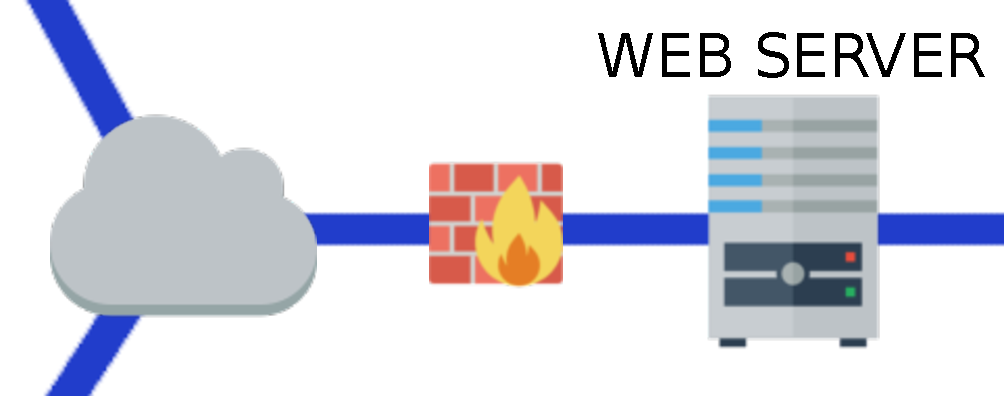
\includegraphics[width=200px]{../Datas/images/firewall.pdf}
	}
	\caption{A firewall}
	\label{fig:firewall}
\end{figure}

	\item \textbf{Demilitarized zone}: since our system is connected to the internet, all the services exposed by the system and used by the system are publicy available and accessible. This is true not only for the web server services but, for instance, even for the database server, which services are used to access and manage data. 

In general, exposing services that directly manage sensitive informations or performe high-risk operations is not a secure choice. One of the most common and reliable architectural choice to increase the security of the system is the creation of a \textit{Demilitarized Zone}, also abbreviated as \textit{DMZ}. In our architecture, a DMZ is created by means of two firewalls, one placed in front of the web server tier, one in front of data tier. This configuration place implicity into the DMZ the web server tier and the application tier.
\begin{figure}[H]
	\centerline{
		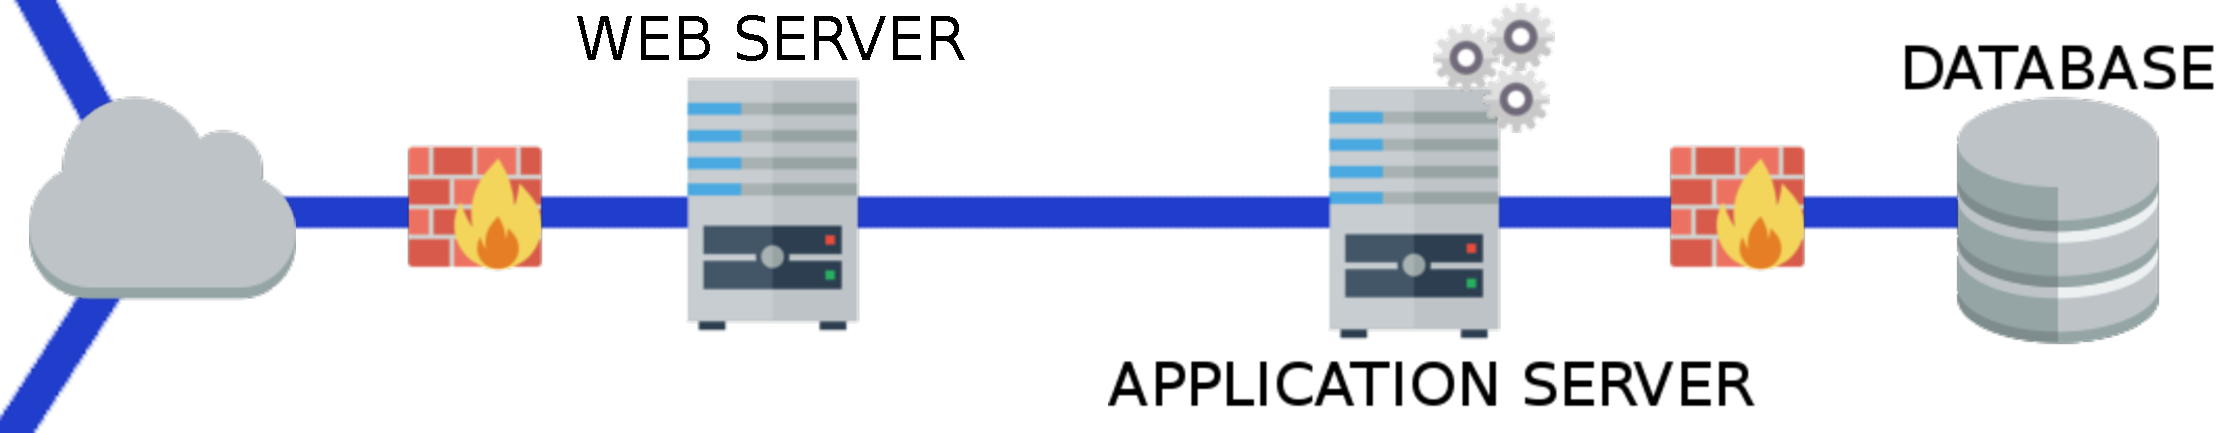
\includegraphics[width=350px]{../Datas/images/dmz.pdf}
	}
	\caption{The Demilitarized Zone}
	\label{fig:dmz}
\end{figure}
	\item \textbf{Stored password protection}: system's breaching and data leakage is a possiblity that can occure even in the most protected environment. To further improve the security of customers' profiles, use of cryptographic hashing algorithms and salting method, are applied to passwords stored into the database.
	\item \textbf{Password security}: to avoid the main typical attack against password, like dictionary attacks and brute-force attacks, the password's characteristics accepted are designed to have minimal lenght of 8 characters, formed alphanumerical and special characters and contains at least one capital letter, one non-capital letter, one digit and one special character.
	\item \textbf{Secure connection}: nowaday everyone can, by means of a device and a packet sniffer, capture, monitor and tamper the internet traffic. Exchange of sensitive informations over the internet can be quite dangerous, either for software systems and users. Thus, the use of communication protocols strongly based on encryption between our software system and the devices (vehicles and user's devices) is required.
	\item \textbf{DoS/DDoS protection}: one of the most dangerous and serious attack for a society providing a service over the internet is the Denial of Service and its Distributed version. To leverage possible attack scenarios involving large volume of traffic from malicious users, firewalls and load balancer are placed at the entry of the software system's network.
\end{itemize}
